\documentclass{ximera}
 

\usepackage{epsfig}

\graphicspath{
  {./}
  {figures/}
}

\usepackage{morewrites}
\makeatletter
\newcommand\subfile[1]{%
\renewcommand{\input}[1]{}%
\begingroup\skip@preamble\otherinput{#1}\endgroup\par\vspace{\topsep}
\let\input\otherinput}
\makeatother

\newcommand{\includeexercises}{\directlua{dofile("/home/jim/linearAlgebra/laode/exercises.lua")}}

%\newcounter{ccounter}
%\setcounter{ccounter}{1}
%\newcommand{\Chapter}[1]{\setcounter{chapter}{\arabic{ccounter}}\chapter{#1}\addtocounter{ccounter}{1}}

%\newcommand{\section}[1]{\section{#1}\setcounter{thm}{0}\setcounter{equation}{0}}

%\renewcommand{\theequation}{\arabic{chapter}.\arabic{section}.\arabic{equation}}
%\renewcommand{\thefigure}{\arabic{chapter}.\arabic{figure}}
%\renewcommand{\thetable}{\arabic{chapter}.\arabic{table}}

%\newcommand{\Sec}[2]{\section{#1}\markright{\arabic{ccounter}.\arabic{section}.#2}\setcounter{equation}{0}\setcounter{thm}{0}\setcounter{figure}{0}}

\newcommand{\Sec}[2]{\section{#1}}

\setcounter{secnumdepth}{2}
%\setcounter{secnumdepth}{1} 

%\newcounter{THM}
%\renewcommand{\theTHM}{\arabic{chapter}.\arabic{section}}

\newcommand{\trademark}{{R\!\!\!\!\!\bigcirc}}
%\newtheorem{exercise}{}

\newcommand{\dfield}{{\sf dfield9}}
\newcommand{\pplane}{{\sf pplane9}}

\newcommand{\EXER}{\section*{Exercises}}%\vspace*{0.2in}\hrule\small\setcounter{exercise}{0}}
\newcommand{\CEXER}{}%\vspace{0.08in}\begin{center}Computer Exercises\end{center}}
\newcommand{\TEXER}{} %\vspace{0.08in}\begin{center}Hand Exercises\end{center}}
\newcommand{\AEXER}{} %\vspace{0.08in}\begin{center}Hand Exercises\end{center}}

% BADBAD: \newcommand{\Bbb}{\bf}

\newcommand{\R}{\mbox{$\Bbb{R}$}}
\newcommand{\C}{\mbox{$\Bbb{C}$}}
\newcommand{\Z}{\mbox{$\Bbb{Z}$}}
\newcommand{\N}{\mbox{$\Bbb{N}$}}
\newcommand{\D}{\mbox{{\bf D}}}
\usepackage{amssymb}
%\newcommand{\qed}{\hfill\mbox{\raggedright$\square$} \vspace{1ex}}
%\newcommand{\proof}{\noindent {\bf Proof:} \hspace{0.1in}}

\newcommand{\setmin}{\;\mbox{--}\;}
\newcommand{\Matlab}{{M\small{AT\-LAB}} }
\newcommand{\Matlabp}{{M\small{AT\-LAB}}}
\newcommand{\computer}{\Matlab Instructions}
\newcommand{\half}{\mbox{$\frac{1}{2}$}}
\newcommand{\compose}{\raisebox{.15ex}{\mbox{{\scriptsize$\circ$}}}}
\newcommand{\AND}{\quad\mbox{and}\quad}
\newcommand{\vect}[2]{\left(\begin{array}{c} #1_1 \\ \vdots \\
 #1_{#2}\end{array}\right)}
\newcommand{\mattwo}[4]{\left(\begin{array}{rr} #1 & #2\\ #3
&#4\end{array}\right)}
\newcommand{\mattwoc}[4]{\left(\begin{array}{cc} #1 & #2\\ #3
&#4\end{array}\right)}
\newcommand{\vectwo}[2]{\left(\begin{array}{r} #1 \\ #2\end{array}\right)}
\newcommand{\vectwoc}[2]{\left(\begin{array}{c} #1 \\ #2\end{array}\right)}

\newcommand{\ignore}[1]{}


\newcommand{\inv}{^{-1}}
\newcommand{\CC}{{\cal C}}
\newcommand{\CCone}{\CC^1}
\newcommand{\Span}{{\rm span}}
\newcommand{\rank}{{\rm rank}}
\newcommand{\trace}{{\rm tr}}
\newcommand{\RE}{{\rm Re}}
\newcommand{\IM}{{\rm Im}}
\newcommand{\nulls}{{\rm null\;space}}

\newcommand{\dps}{\displaystyle}
\newcommand{\arraystart}{\renewcommand{\arraystretch}{1.8}}
\newcommand{\arrayfinish}{\renewcommand{\arraystretch}{1.2}}
\newcommand{\Start}[1]{\vspace{0.08in}\noindent {\bf Section~\ref{#1}}}
\newcommand{\exer}[1]{\noindent {\bf \ref{#1}}}
\newcommand{\ans}{}
\newcommand{\matthree}[9]{\left(\begin{array}{rrr} #1 & #2 & #3 \\ #4 & #5 & #6
\\ #7 & #8 & #9\end{array}\right)}
\newcommand{\cvectwo}[2]{\left(\begin{array}{c} #1 \\ #2\end{array}\right)}
\newcommand{\cmatthree}[9]{\left(\begin{array}{ccc} #1 & #2 & #3 \\ #4 & #5 &
#6 \\ #7 & #8 & #9\end{array}\right)}
\newcommand{\vecthree}[3]{\left(\begin{array}{r} #1 \\ #2 \\
#3\end{array}\right)}
\newcommand{\cvecthree}[3]{\left(\begin{array}{c} #1 \\ #2 \\
#3\end{array}\right)}
\newcommand{\cmattwo}[4]{\left(\begin{array}{cc} #1 & #2\\ #3
&#4\end{array}\right)}

\newcommand{\Matrix}[1]{\ensuremath{\left(\begin{array}{rrrrrrrrrrrrrrrrrr} #1 \end{array}\right)}}

\newcommand{\Matrixc}[1]{\ensuremath{\left(\begin{array}{cccccccccccc} #1 \end{array}\right)}}



\renewcommand{\labelenumi}{\theenumi)}
\newenvironment{enumeratea}%
{\begingroup
 \renewcommand{\theenumi}{\alph{enumi}}
 \renewcommand{\labelenumi}{(\theenumi)}
 \begin{enumerate}}
 {\end{enumerate}\endgroup}



\newcounter{help}
\renewcommand{\thehelp}{\thesection.\arabic{equation}}

%\newenvironment{equation*}%
%{\renewcommand\endequation{\eqno (\theequation)* $$}%
%   \begin{equation}}%
%   {\end{equation}\renewcommand\endequation{\eqno \@eqnnum
%$$\global\@ignoretrue}}

%\input{psfig.tex}

\author{Martin Golubitsky and Michael Dellnitz}

%\newenvironment{matlabEquation}%
%{\renewcommand\endequation{\eqno (\theequation*) $$}%
%   \begin{equation}}%
%   {\end{equation}\renewcommand\endequation{\eqno \@eqnnum
% $$\global\@ignoretrue}}

\newcommand{\soln}{\textbf{Solution:} }
\newcommand{\exercap}[1]{\centerline{Figure~\ref{#1}}}
\newcommand{\exercaptwo}[1]{\centerline{Figure~\ref{#1}a\hspace{2.1in}
Figure~\ref{#1}b}}
\newcommand{\exercapthree}[1]{\centerline{Figure~\ref{#1}a\hspace{1.2in}
Figure~\ref{#1}b\hspace{1.2in}Figure~\ref{#1}c}}
\newcommand{\para}{\hspace{0.4in}}

\renewenvironment{solution}{\suppress}{\endsuppress}

\ifxake
\newenvironment{matlabEquation}{\begin{equation}}{\end{equation}}
\else
\newenvironment{matlabEquation}%
{\let\oldtheequation\theequation\renewcommand{\theequation}{\oldtheequation*}\begin{equation}}%
  {\end{equation}\let\theequation\oldtheequation}
\fi

\makeatother

\begin{document}

\noindent In Exercises~\ref{c9.6.4a} -- \ref{c9.6.4c}, consider the system 
of differential equations \eqref{E:twoeq}
\begin{matlabEquation}  \label{E:twoeq}
\begin{array}{rcl}
\dot{x} & = & y - x + (x-\rho)^2 \\
\dot{y} & = & y - x^3 +3x
\end{array}
\end{matlabEquation}
in the square $-5 \leq x,y \leq 5$.
\begin{computerExercise} \label{c9.6.4a}
How many equilibria does \eqref{E:twoeq} have in this square when 
$\rho=1.7$ and of what type are they?  This question can be answered either 
numerically using {\pplane} (easy) or analytically (more difficult, but 
possible).

\begin{solution}

\ans The system has a saddle at $(x,y) \approx (0.4,-1.2)$, and a 
spiral source at $(x,y) \approx (2.0,1.9)$.

\soln Either determine the equilibria numerically from the {\tt pplane5}
graph of the system (Figure~\ref{c9.6.4b}a), or compute analytically.  To
do this, solve $\dot{y} = 0$ to find that $y = x^3 - 3x$ at all equilibria.
Then, substitute this value for $y$ into $\dot{x}$ and solve $\dot{x} = 0$
to obtain $0 = x^3 + x^2 - 7.4x + 2.89$.  Find the roots of this equation
to confirm that $(x,y) \approx (0.4,-1.2)$ and $(x,y) \approx (2.0,1.9)$
are equilibria.  There is a third equilibrium at $(x,y) \approx
(-3.4,-29)$ which is not in the graph range.

\para The general Jacobian for the system is
\[
J = \cmattwo{-1 + 2(x - \rho)}{1}{-3x^2 + 3}{1}.
\]
Thus, when $\rho = 1.7$, $\trace(J) = 2(x - 1.7)$ and
$\det(J) = 3x^2 + 2(x - 1.7) - 4$.  At $(x,y) \approx (0.4,-1.2)$,
$\det(J) \approx -6.1 < 0$, so the equilibrium is a saddle.  At
$(x,y) \approx (2.0,1.9)$, $\det(J) \approx 8.6 > 0$, $\trace(J) \approx
0.6 > 0$, and $D = (\trace(J))^2 - t\det(J) \approx -34 < 0$.  Therefore,
this equilibrium is a spiral source.

\end{solution}
\end{computerExercise}
\begin{computerExercise} \label{c9.6.4b}
What type of bifurcation occurs in \eqref{E:twoeq} as $\rho$ is varied
from $\rho=1.7$ to $\rho=1.85$?

\begin{solution}
A homoclinic bifurcation occurs between $\rho = 1.7$ and
$\rho = 1.85$.  As $\rho$ increases from $\rho = 1.7$, an unstable
orbit of the saddle point crosses a stable orbit of the saddle.  After
this point, there is a periodic solution around the spiral source.

\end{solution}
\end{computerExercise}
\begin{computerExercise} \label{c9.6.4c}
What type of bifurcation occurs in \eqref{E:twoeq} as $\rho$ is varied
from $\rho=1.85$ to $\rho=2.1$?

\begin{solution}
A Hopf bifurcation occurs between $\rho = 1.85$ and
$\rho = 2.1$.  The spiral source passes through a center and becomes a
spiral sink.  At this point, the periodic solution disappears.

Figure~\ref{c9.6.4b}a shows the system with $\rho = 1.7$.
Figure~\ref{c9.6.4b}b shows the system with $\rho = 1.85$.
Figure~\ref{c9.6.4b}c shows the system with $\rho = 2.1$.

\begin{figure}[htb]
                       \centerline{%
                       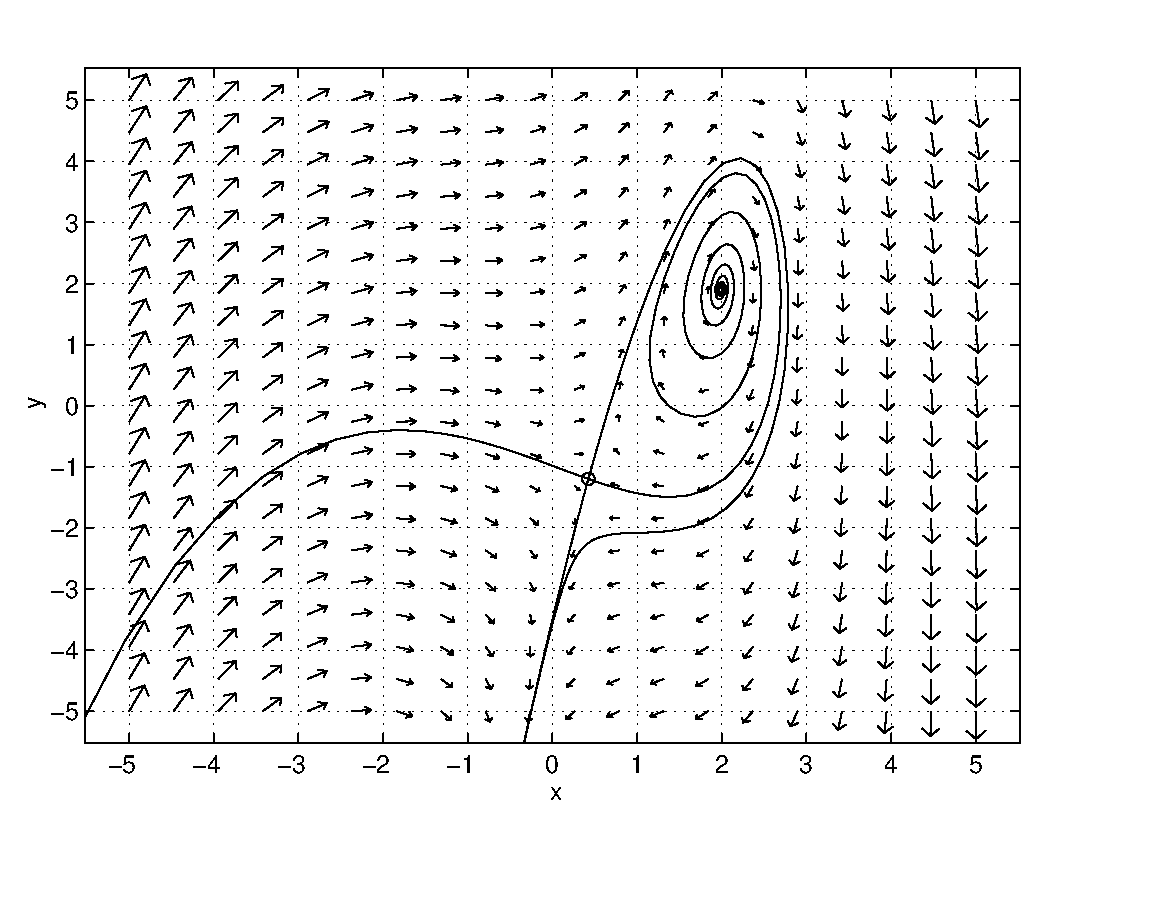
\psfig{file=exfigure/9-6-4a.eps,width=1.8in}
                       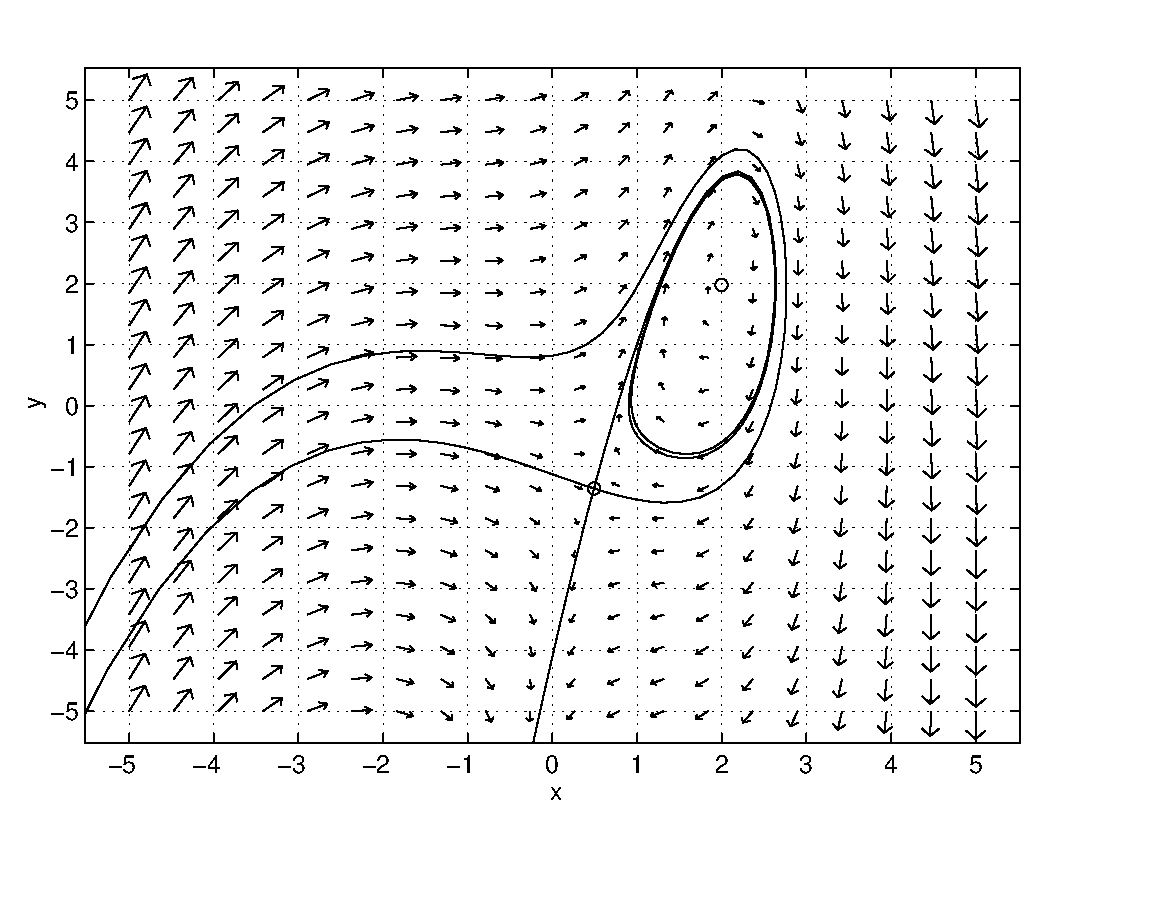
\psfig{file=exfigure/9-6-4b.eps,width=1.8in}
                       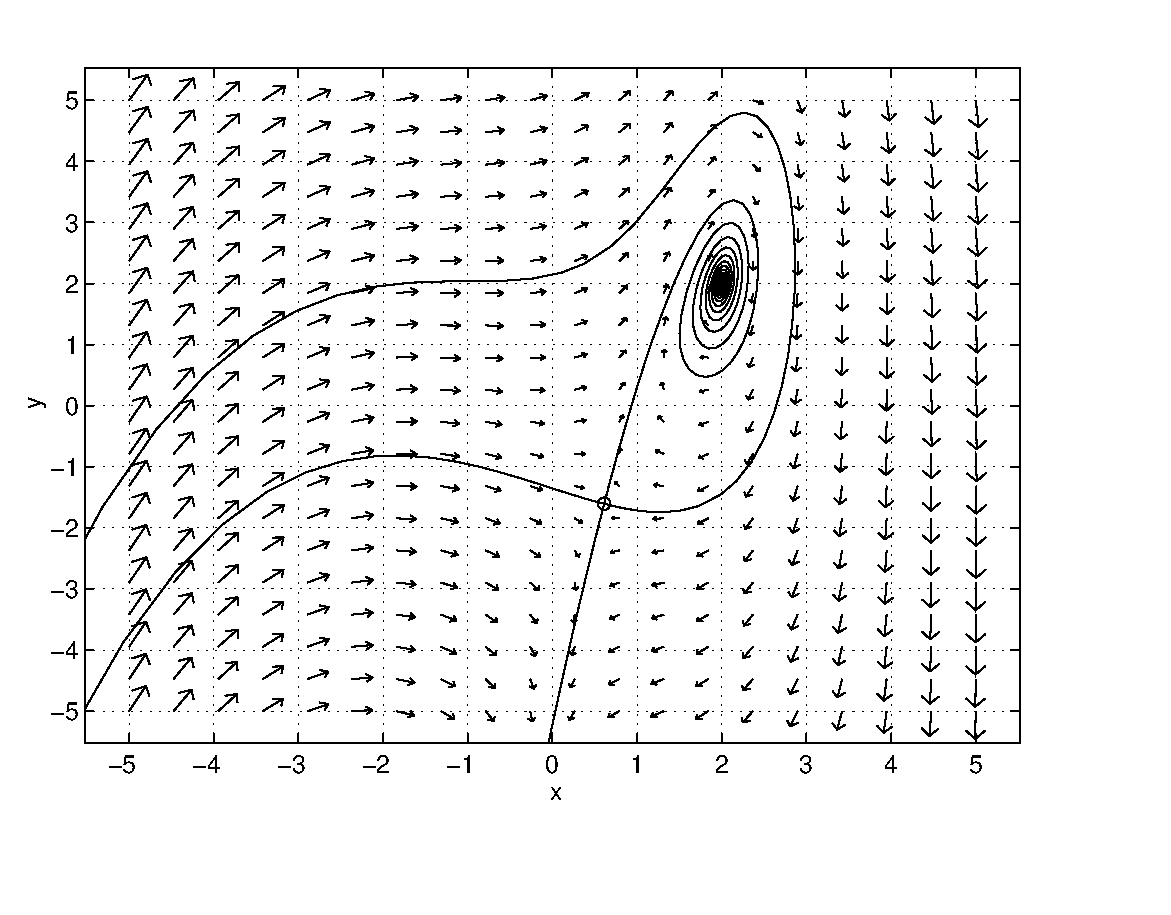
\psfig{file=exfigure/9-6-4c.eps,width=1.8in}}
		\centerline{$\rho = 1.7$\hspace{1.3in}$\rho = 1.85$
\hspace{1.3in}$\rho = 2.1$}
                \exercapthree{c9.6.4b}
\end{figure}


\end{solution}
\end{computerExercise}
\end{document}
